\chapter{Execução da Pesquisa}


\section{Ferramentas usadas}

O código será versionado no
Github\footnote{\url{https://github.com/diegofreitas/platform_packages_apps_contacts}}
onde será feito o gerenciamento das versões de cada iteração.
As ferramentas utilizadas para a refatoração serão a IDE Eclipse(Juno) com
plugin ADT v21 para facilitar a edição do código e ferramentas de construção
do projeto existentes no próprio repositório do android tendo em vista que todo
o processo de compilação e empacontamento não visa ser usado em uma ide.
Para fazer a coleta das métricas é necessario que a ferramenta analise código
java e contemple todas as métricas descritas na seção \ref{sec:metrics}. O
programa Chidamber and Kemerer Java
Metrics\footnote{\url{https://github.com/dspinellis/ckjm}} atende esses
critérios, além de ser um projeto de código-aberto.

\section{Análise do objeto de estudo}

O aplicativo a ser refatorado tem funcionalidades para gerenciamento de
contatos. Dentro deste conjunto de casos de uso será feratorado o pacote
referente ao gerenciamento de grupos de contatos presente no pacote
\textbf{com.android.contacts.group} que contém componentes de tela para
interação com o usuário a saber:
\begin{description}
\item[GroupDetailFragment.java] Exibe os dados de um grupo de contatos.
\item[GroupBrowseListFragment.java] Fonece uma lista de grupos.
\item[GroupEditorFragment.java] Disponibiliza um formulário para edição dos
dados de um grupo.
\end{description}

Estas intefaces são usadas dentro de activities que controlam uma parte do fluxo
de interação e se comportam de forma diferente conforme o tipo de dispositivo
móvel utilizado. Devido a essa complexidade, não será feita nenhuma alteração na
interface pública dos componentes refatorados evitando efeitos colaterais em
outras partes do aplicativo.

Os componetes elencados contém código não somente relacionado com a lógica de
apresentação como também interagem diretamente com classes destinadas ao acesso
de dados e serviços existentes nas dependências do projeto, por exemplo,
gerenciamento de contas do usuário. 

Cada iteração compreenderá na na refatoração de cada um dos componentes
descritos. O marco de referência de dados das métricas presentes na tabela \ref{tab:dados_baseline} será feita a partir da
versão \verb|4.4.2_r1| do aplicativo.

\begin{table}[h]
	\centering
    \begin{tabular}{ | l | l | }
    \hline
    Métrica &	Média \\ \hline
    WMC  	&	8.5161290323   	\\ \hline
    DIT	 	&	0.7741935484	\\ \hline
	NOC  	& 	0				\\ \hline
	CBO	  	& 	10.1612903226	\\ \hline
	RFC	 	& 	23.7419354839	\\ \hline
	LCOM 	& 	57.4838709677	\\ \hline
    \end{tabular}
    \caption{Métricas CK para linha de base}
    \label{tab:dados_baseline}
\end{table}

\section{Arquitetura Proposta}

Será aplicado nos experimentos a variação do padrão MVP chamada Passive View,
pois dessa forma, o Model não precisa publicar alterações de seu estado para a
view, dessa forma evita-se alterações no código referente às classes que fazem
parte da camada de Model do aplicativo de contatos. A organização do código
fonte no repositório dificulta a implementação porque esses componentes estão
localizados fora do projeto afetado e são compartilhados.

As classes que extendem Fragment terão a responsabilidade da View pois é neste
componente que a interface com o usuário é construída. A classe Activity fornece
vários métodos para recuperação de recursos de imagens, textos, inicialização de
serviços, entre outros. Isso ocorre porque a classe Activity é uma subclasse de Context, herdando diversos métodos não relacionados ao gerenciamento da interface.

Segundo \citeonline{Reenskaug:1979} ``\ldots Os papéis da View e o
Controller podem ser exercidos pelo mesmo objeto quando eles estão muito
acoplados. Exemplo: A Menu.'', porém isso requer um boa análise do problema em
questão para decidir o nível de granularidade que esses componentes podem ter.
Portanto, é recomendável manter sempre essa separação para manter uma boa coesão
nas classes. O Presenter será uma classe auxiliar à view e pode ser implementada
como uma classe java simples. 



\section{Experimentos}



\subsection{WMC}

Como fazer referência à tabela e ao gráfico?
\begin{table}[h]
	\centering
    \begin{tabular}{ | l | l | }
    \hline
    Iteração & Média 			\\ \hline
    Baseline & 8.5161290323   	\\ \hline
    Iteração 1 & 8.875			\\ \hline
	Iteração 2 & 9				\\ \hline
	Iteração 3 & 8.9393939394	\\ \hline
    \end{tabular}
    \caption{Valores da métrica}
    \label{tab:dados_iteracao1}
\end{table}

\begin{figure}[h]
	\centering
	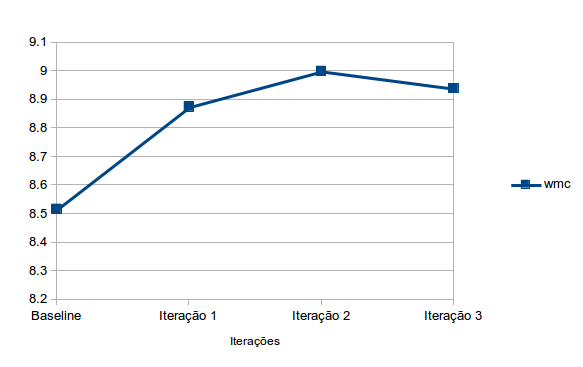
\includegraphics{img/wmc.png}
	\caption{Gráfico da métrica WMC/Fonte: Próprio autor} 
	\label{fig:wmc}
\end{figure}


Segundo \citeonline{cksuite} “. . . The larger the number of methods in
a class the greater the potential impact on children, since children will inherit all the
methods defined in the class. . . . Classes with large numbers of methods are likely to
be more application specific, limiting the possibility of reuse.” as classes analisadas
são de interface, portanto implementão uma interação com o usuário bem
específica que não serão reutilizadas por meio de herança.

\subsection{DIT}


A figura \ref{fig:dit} mostrar um aumento no valor da métrica DIT, que deve ser
mantido baixo pois quanto mais abaixo na hierarquia de heraça a classe estiver, menos previsível será seu
comportamento devido a quantidade de classes acima, entretanto o aumento no DIT
se deve ao fato que o ckjm considera a implementação de interface como herança.
A interface define somente o contrato que a classe de implementar não havendo
nenhuma implementação que pudesse interferir no comportamento da classe,
portanto essa alteração no DIT não deve ser considerada.

\begin{figure}[h]
	\centering
	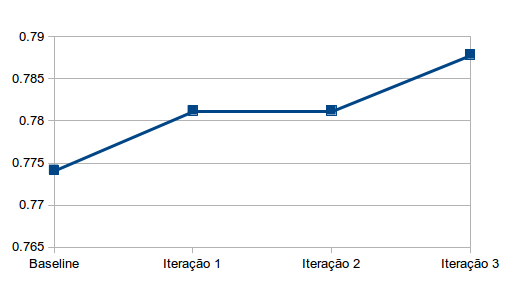
\includegraphics{img/dit.png}
	\caption{Valores de DIT/Fonte: Próprio autor}
	\label{fig:dit}
\end{figure}


\subsection{NOC}

Nenhuma classe foi herdada para a aplicação do padrão, portanto, essa métrica
permaneceu intacta durante as iterações.

\begin{figure}[h]
	\centering
	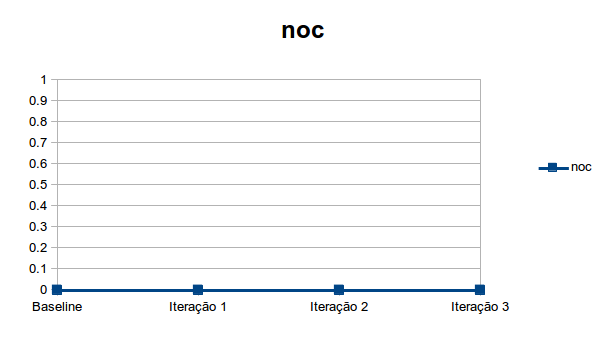
\includegraphics{img/noc.png}
	\caption{Valores de NOC/Fonte: Próprio autor}
	\label{fig:noc}
\end{figure}

\subsection{CBO}

Na primeira iteração foi aplicado o padrão em um componente mais simples e foi
possível remover qualquer dependência que não fosse relacionada a interface,
entretanto, a maior queda ocorreu em  ficando a cargo do da experiência do
desenvolvedor identificar estes cenários específicos. Nas iterações seguintes as
interfaces alteradas são mais complexos,


\begin{figure}[h]
	\centering
	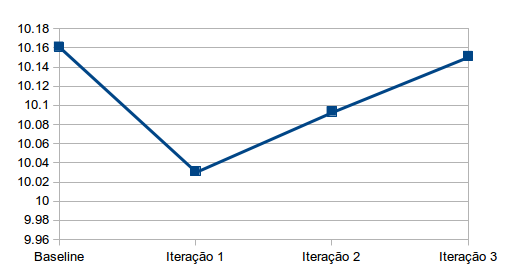
\includegraphics{img/cbo.png}
	\caption{Valores de CBO/Fonte: Próprio autor}
	\label{fig:cbo}
\end{figure}


\subsection{RFC}

A métrica RFC tende a aumentar a cada iteração o que sugere um aumento da
complexidade do código conforme é apresentado na Figura \ref{fig:rfc}.

\begin{figure}[h]
	\centering
	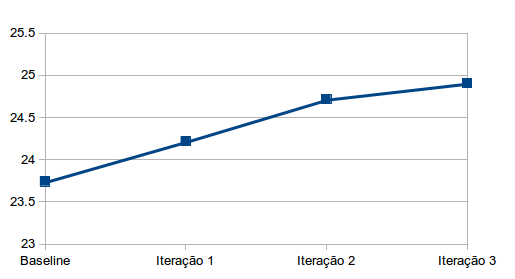
\includegraphics{img/rfc.png}
	\caption{Valores de RFC/Fonte: Próprio autor}
	\label{fig:rfc}
\end{figure}



\subsection{LCOM}

\begin{figure}[h]
	\centering
	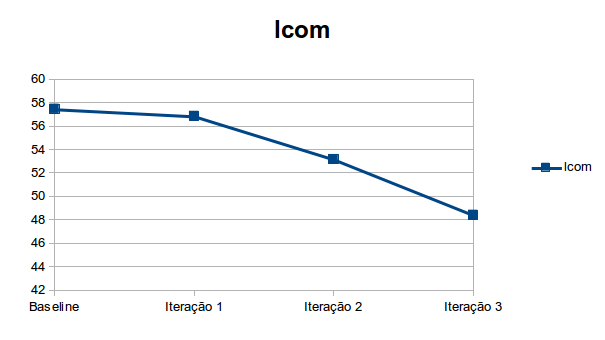
\includegraphics{img/lcom.png}
	\caption{Valores de lcom/Fonte: Próprio autor}
	\label{fig:lcom}
\end{figure}

A Figura \ref{fig:lcom} mostra uma queda siginificativa na métrica LCOM. Isto
indica que a coesão do código melhorou após cada iteração. 


